
\documentclass[brazilian,12pt,a4paper,final]{article}


\usepackage[a4paper,
bindingoffset=0.2in,
left=0.8in,
right=0.8in,
top=0.8in,
bottom=0.8in,
footskip=.25in]{geometry}

%% Pacotes extras (opcionais):

% *babel* contem as regras de hifenização
\usepackage[portuguese]{babel}
% *t1enc* permite o reconhecimento dos acentos inseridos com o teclado
\usepackage{t1enc}

% *inputenc* com opção *utf8* permite reconhecimento dos caracteres com codificação UTF8, que é padrão dos esditores de texto no Linux. Isso permite reconhecimento automático de acentuação.
%\usepackage[utf8]{inputenc}
\usepackage{epsfig}

% *graphicx* é para incluir figuras em formato eps 
\usepackage{graphicx} % para produzir PDF diretamente reescrever esta linha assim: \usepackage[pdftex]{graphicx}

% *color* fontes soloridas
\usepackage{color}
%%% fim do cabecalho %%%

\pagestyle{empty}
\title{Métodos Computacionais Aplicados à Biocomplexidade}
\author{Aluno: André Gustavo Dessoy Hubner - Matrícula: 00315569 \\ IF-UFRGS}

\begin{document}
	\maketitle
	
	\section{Introdu\c{c}\~ao} 
	% Aqui a Introdução \c{c} e \~a  é a forma standar  de escrever
	% carateres ASCII extendidos (acentos, etc), porem com o pacote t1enc
	% declarado acima podemos escrever diretamente ç em lugar d \c{c}, etc
	\indent 
	Este documento relata os resultados obtidos da modelagem de um sistema biológico visto em aula através de equações diferenciais, assim como observações advindas do estudo de simulações deste.
	
	\section{Metodologia}
	\subsection{Modelagem das reações químicas e funções de Hill}
	O sistema biológico modelado aqui, assim como a equação diferencial que o representa, estão representados nas duas primeiras figuras. Alguns pontos importantes podem ser levantados:
	
	\begin{figure}[hbtp]
		\begin{center}
			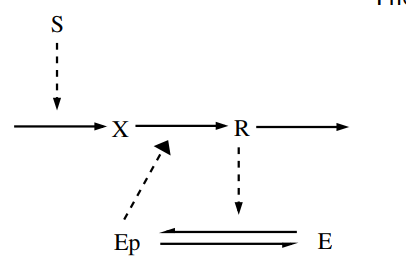
\includegraphics[]{Reações.png}
			\caption{Série de reações do sistema biológico.}
			\label{fig}
		\end{center}
	\end{figure}
	
	\begin{figure}[hbtp]
		\begin{center}
			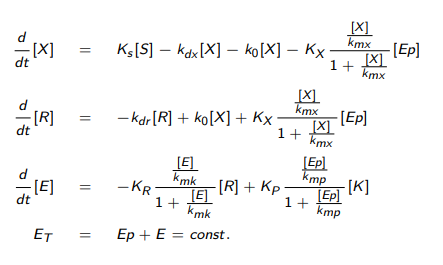
\includegraphics[]{Equações.png}
			\caption{Equações diferenciais modelando o sistema.}
			\label{fig}
		\end{center}
	\end{figure}
	
	\begin{itemize}
		\item S, de concentração constante, ativa a produção de X
		\item X por sua vez está diretamente responsável pela formação de R em uma reação ajudada por Ep (E em sua forma fosforilada)
		\item R atua como quinase em E, convertendo-o em Ep
		\item Já a conversão de Ep em E é feita por K (não representado na figura), também de concentração constante
	\end{itemize}
	
	Para adaptar essa modelagem ao código, o primeiro passo envolveu a criação das funções de hill. Essas funções são essenciais para modelar as variações das concentrações dos compostos advindas de ações enzima-ligante, uma vez que a função de ativação de Hill, por exemplo, retorna justamente uma variação correspondente à ação da enzima com o composto precursor para formar o composto produto. A função de inibição de Hill também foi adaptada, mesmo que não tenha sido utilizada.
	\vspace{0.5cm}
	
	Em seguida, preparei um dicionário contendo chaves correspondentes a todos os parâmetros necessários para representar as equações em códigos e executar as simulações. Neste dicionário são definidos todos os valores das taxas de formação e degradação dos compostos, todas as constantes de Michaelis-Mentes das respectivas reações, as concentrações iniciais de todos os compostos do sistema e os tempos iniciais, finais e de variação por uma simulação. Optei por centralizar tudo em uma estrutura pois facilita a mudança rápida das características do sistema da próxima execução, além de poder explicar a função de cada variável em uma só página.
	\vspace{0.5cm}
	
	E então, finalmente modelando uma rodada de interações do sistema, construí a função "Simulation". Ela recebe apenas o dicionário do passo anterior, atribuindo o valor de cada chave dele a variáveis locais e criando listas para armazenar as variações dos compostos não constantes (X, R e E), além de uma para armazenar cada instante de tempo. A partir disso, inicia-se um laço while que só será finalizado ao tempo atingir o limite especificado, e em cada iteração será calculado o incremento assim como especificado nas equações da figura 4, sendo estas traduzidas e adaptadas ao código. O incremento total é dependente e diretamente proporcional do valor de dt definido nos parâmetros. Ao terminar o laço, a função termina retornando todas as listas preenchidas.
	As oscilações resultantes da aplicação desta função às configurações utilizadas serão demonstradas na seção de resultados.
	
	\begin{figure}[hbtp]
		\begin{center}
			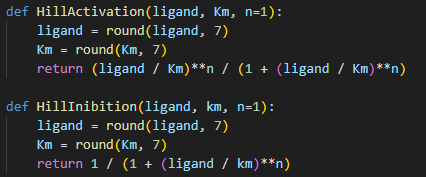
\includegraphics[width=14cm]{Hill.png}
			\caption{Funções de Hill adaptadas para o código.}
			\label{fig}
		\end{center}
	\end{figure}
	
	\begin{figure}[hbtp]
		\begin{center}
			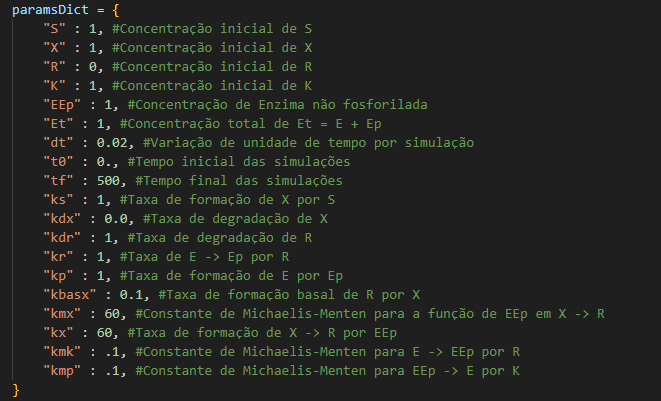
\includegraphics[height=10cm, width=14cm]{dict.png}
			\caption{Dicionário com todas as variáveis parametrizáveis usadas na simulação do sistema biológico. Os valores representados aqui foram os primeiros a serem utilizados.}
			\label{fig}
		\end{center}
	\end{figure}
	
		\begin{figure}[hbtp]
		\begin{center}
			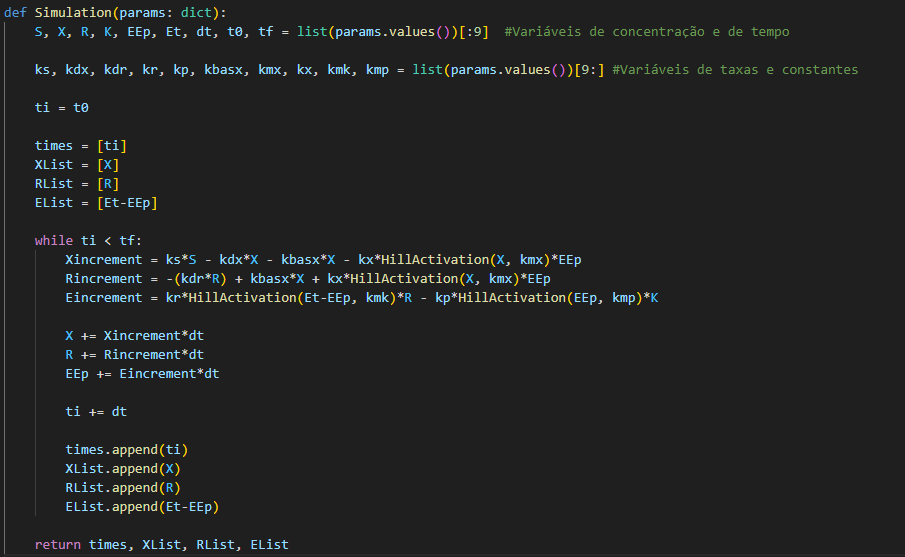
\includegraphics[height=10cm, width=14cm]{Simulation.png}
			\caption{Função que realiza uma rodada de Simulação para os parâmetros específicados.}
			\label{fig}
		\end{center}
	\end{figure}

	
	\subsection{Obtenção dos períodos das oscilações}
	Para obter os períodos das oscilações, criei primeiro uma função "ExtractMaximals", que recebendo todas as listas provenientes de uma execução de Simulation, retorna ao todo 6 listas, sendo para cada composto de concentração variável uma contendo todos os seus pontos de máximo e outra os tempos de cada um destes instantes. Separando os retornos dessa maneira, seria fácil plotar os pontos de máximo de cada composto.
	\vspace{0.5cm}
	
	Em seguida criei a função "ExtractPeriodsMeans", que recebendo as listas dos tempos dos pontos maximais de cada composto retorna a média dos períodos entre as oscilações de cada unidade. Essa função chama internamente outra função "CalculatePeriods"\ três vezes, esta que realiza a lógica de iterar por toda a lista do parâmetro armazenando em outra lista a diferença de tempo entre cada sucessivo maximal, retornando por fim a média aritmética de todos esses elementos.
	
	\begin{figure}[hbtp]
		\begin{center}
			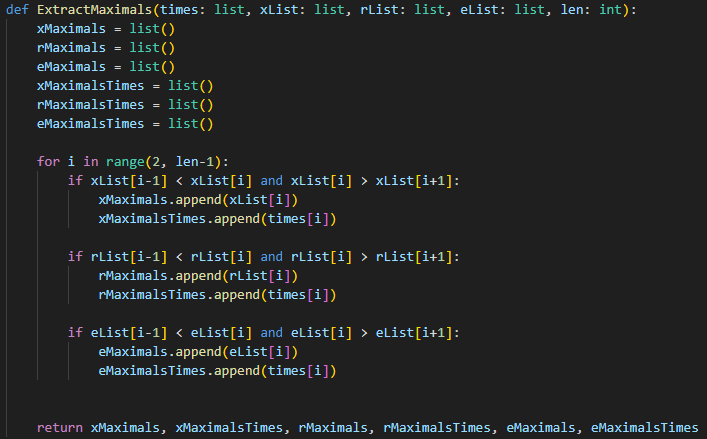
\includegraphics[height=10cm, width=14cm]{ExtractMaximals.png}
			\caption{Função que extrai os pontos maximais assim como o instante de tempo em que eles ocorreram de cada composto.}
			\label{fig}
		\end{center}
	\end{figure}
	
	\begin{figure}[hbtp]
		\begin{center}
			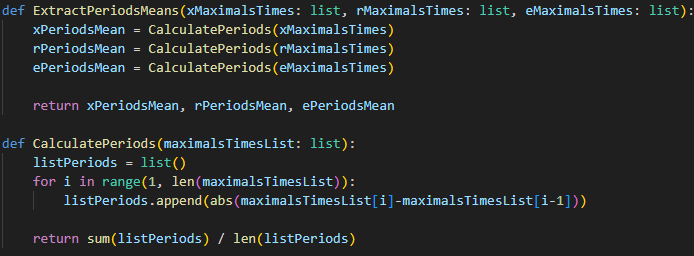
\includegraphics[]{ExtractPeriods.png}
			\caption{Função que retorna a média dos períodos de oscilação de cada composto, chamando CalculatePeriods interanamente para calcular a média em cada composto.}
			\label{fig}
		\end{center}
	\end{figure}
	
	\subsection{Estudo da variação dos parâmetros}
	
	Já para estudar a variação dos períodos do gráfico de acordo com a mudança dos parâmetros foram necessárias várias adaptações. De forma a rodar as simulações com valores diferentes para cada parâmetro de forma rápida e linearizada, comecei a construir a função "SearchPeriods", que gera um array com vários valores entre 0.07 e 2.11 e, para cada um desses valores e para cada parâmetro cabível de modificação do dicionário original, realiza a simulação e os cálculos dos seus períodos, retornando ao final os resultados que fossem suficientemente diferentes.
	\vspace{0.5cm}

	Posteriormente, feitos os primeiros testes dessa função decidi usar a mesma abordagem só que com um array com valores negativos, para obter resultados dos parâmetros com seus valores diminuídos e portanto gerar dados mais diversos. Neste contexto primeiro adaptei SearchPeriods para conter a lógica de utilização desses valores negativos, e depois gerei uma função "SearchLowerUpperPeriods", que chamará ambas as execuções de SearchPeriods, retornando os resultados de ambas em um só array. Esta função também cuida dos parâmetros passados para essas execuções, o que pode ser observado melhor nas figuras 8, 9 e 10.
	
	\begin{figure}[hbtp]
		\begin{center}
			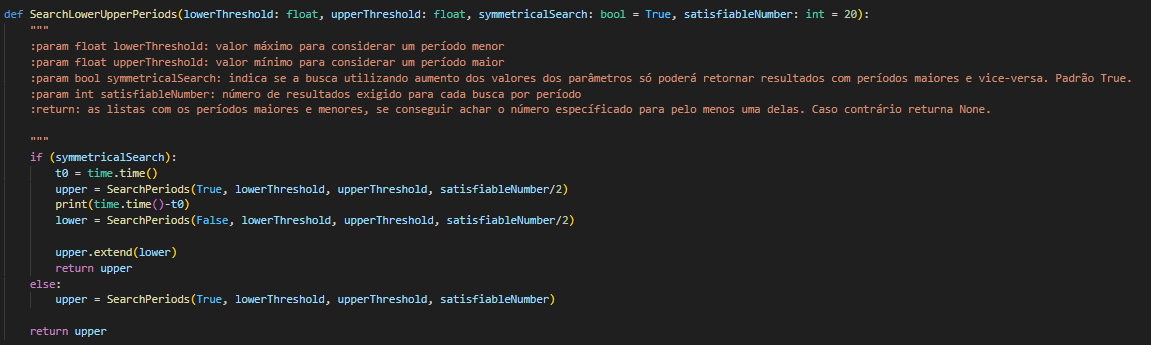
\includegraphics[width=16cm]{SearchLowerUpperPeriods.png}
			\caption{Função que chama as duas execuções de SearchPeriods, uma utilizando valores crescentes e outra decrescentes para cada parâmetro válido.}
			\label{fig}
		\end{center}
	\end{figure}
	
	\begin{figure}[hbtp]
		\begin{center}
			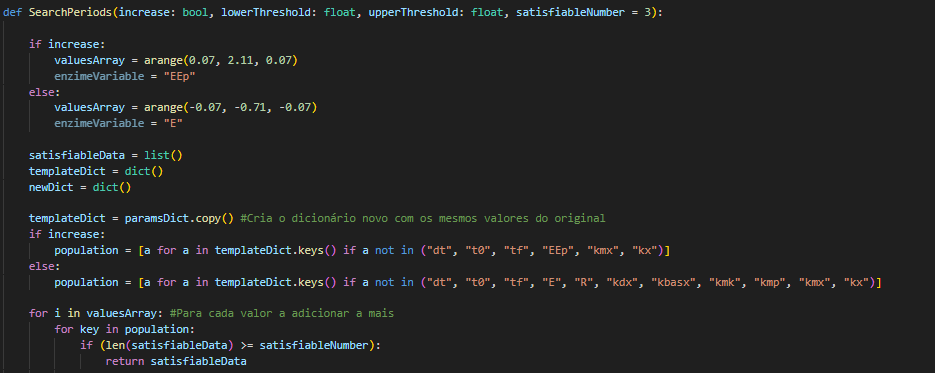
\includegraphics[width=16cm]{SearchPeriods1.png}
			\caption{Primeira parte da função SearchPeriods.}
			\label{fig}
		\end{center}
	\end{figure}
	
	\begin{figure}[hbtp]
		\begin{center}
			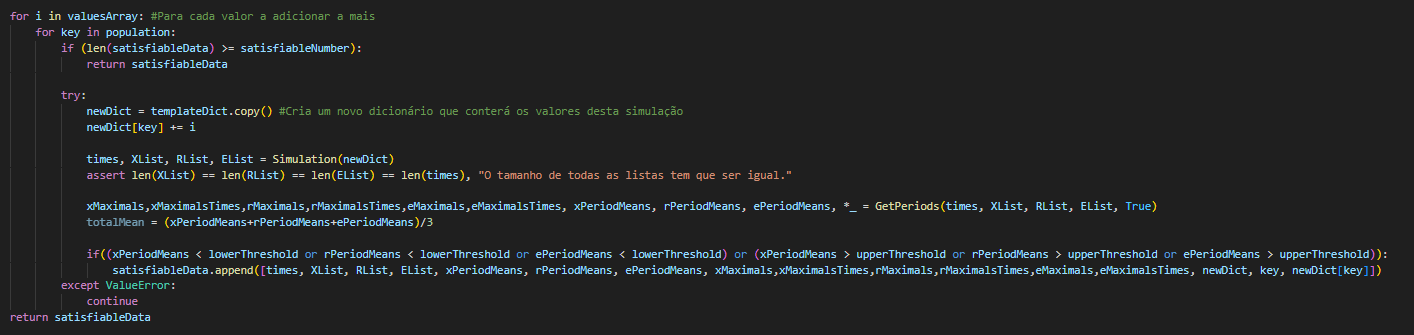
\includegraphics[width=16cm]{SearchPeriods2.png}
			\caption{Segunda parte da função SearchPeriods.}
			\label{fig}
		\end{center}
	\end{figure}
	
	\begin{figure}[hbtp]
		\begin{center}
			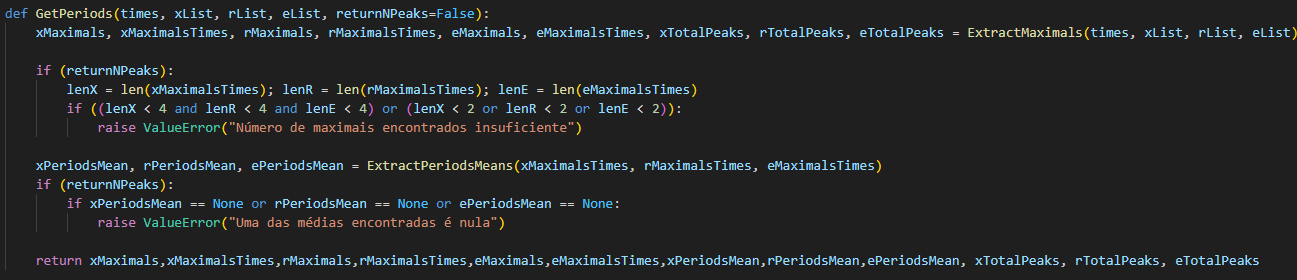
\includegraphics[width=16cm]{GetPeriods.png}
			\caption{Função que encapsula ExtractMaximals e ExtractPeriodMeans, aceitando apenas resultados válidos caso seja chamada a partir do fluxo em que eu estava trabalhando.}
			\label{fig}
		\end{center}
	\end{figure}
	
	Outra adaptação realizada nessa etapa foi a centralização das funções ExtractMaximals e ExtractPeriodMeans na nova função "GetPeriods", para que fosse possível chamar apenas uma função para realizar toda a lógica necessária em SearchPeriods. Além disso, esta função também serviu para encapsular a validação de resultados relevantes para a análise posterior, assim como a exclusão de casos que ocasionariam erro.
	
	\section{Resultados}
	\subsection{Caso inicial}
	
	\begin{figure}[hbtp]
		\begin{center}
			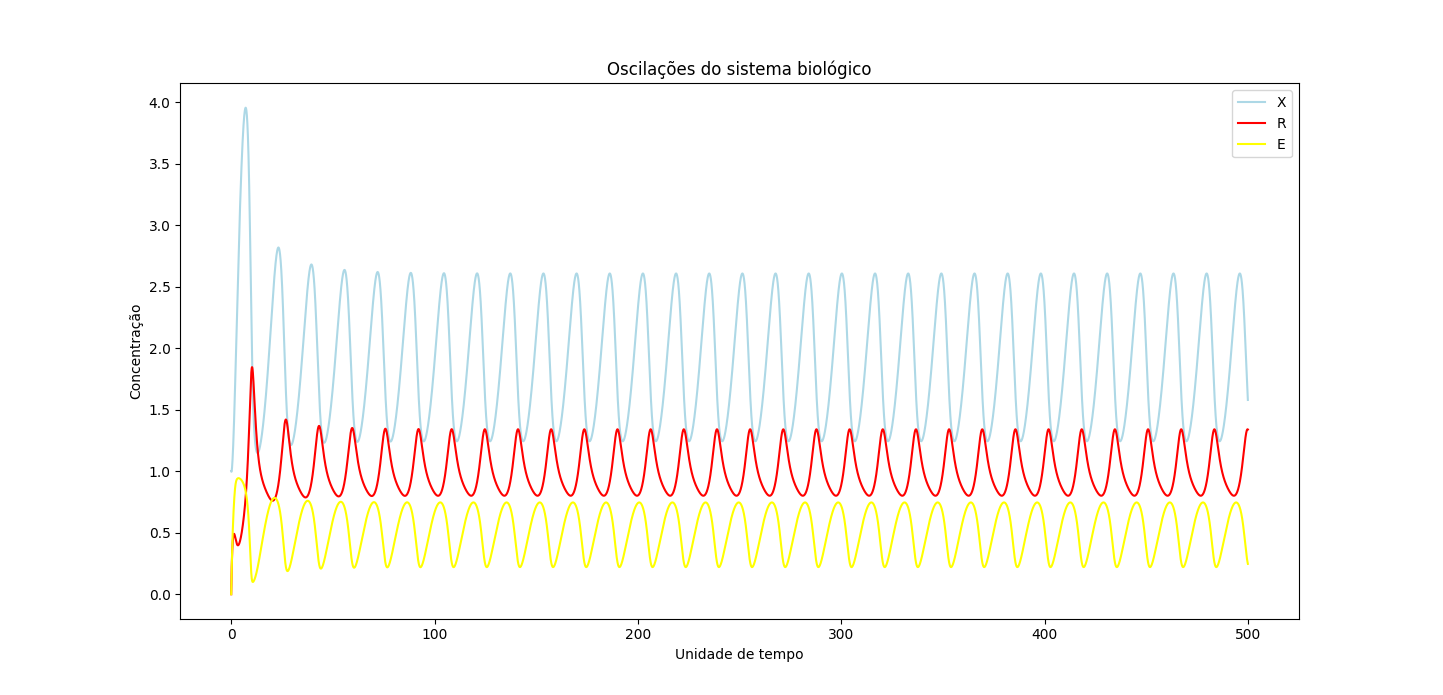
\includegraphics[height=12cm, width=18cm]{oscPadrao.png}
			\caption{Gráfico representando a primeira rodada de oscilações testada. É bastante notável o crescimento vertiginoso da concentração de X, R e E nas primeiras unidades de tempo. Contudo, após o primeiro pico de X e E e o segundo de R, o sistema se estabiliza rapidamente, com oscilações entre concentrações mínimas e máximas praticamente constantes para cada composto}
			\label{fig}
		\end{center}
	\end{figure}
	
	Logo após terminar a criação da função de simulação, executei uma rodada de simulações, chamando a função Simulation e plotando os resultados, que resultaram no gráfico da figura 12. Seus resultados foram interessantes, confirmando o padrão oscilatório de sistemas biológicos envolvendo uma série de regulações entre os próprios membros. Em especial, com apenas X começando em  enquanto R e E começam em 0, dá para se estimar as seguintes razões para o comportamento de cada um:
	
	\begin{itemize}
		\item X tem seu acúmulo muito favorecido por kdx e kbasx, que reduzem sua quantidade, estarem em valores muito baixos (ou zero no segundo), e por kx e kmx se contrabalancearem na ativação da rota X -> R por EEp, enquanto que a taxa de formação de X a partir de S tem o valor de 1 e uma quantidade constante de S para transformar em X;  
		\item A taxa de degradação de R por sua vez tem um valor alto; ainda assim, R consegue crescer pois este é o único ponto que reduz a sua quantidade, enquanto que há taxas basais e de ativação de X -> R formando este composto
		\item E está em equilíbrio com o seu estado fosforilado, e uma vez que começa com 0 em estado desfosforilado, há muito mais composto para formá-lo do que o estado fosforilado, que começa saturado; o efeito vertiginoso do início é amplificado pela presença constante de K, e o sistema acaba equilibrando pela maior presença de R para fosforilá-lo em EEp
	\end{itemize}

	Após maiores refinamentos, incluindo a construção das funções para obter os períodos, atualizei também a plotagem destacando seus pontos de máximo, assim como o período médio entre as oscilações de cada composto (figura 13). 
	
	\begin{figure}[hbtp]
		\begin{center}
			\includegraphics[height=12cm, width=18cm]{Resultado-padrão.png}
			\caption{O mesmo resultado que o de antes, porém destacando os pontos de máximo e informando o período médio entre oscilações de cada composto. O período médio considerando todos os compostos foi de 16.24}
			\label{fig}
		\end{center}
	\end{figure}
	
	\subsection{Estudo do período das oscilações}
	
	Já para estudar a variação dos períodos do gráfico de acordo com a mudança dos parâmetros, foram necessárias várias adaptações, como é possível ver na subseção "Estudo da variação dos parâmetros".
	Para tentar gerar resultados relevantes no mundo real, chamei a SearchLowerUpperPeriods com valores de lowerThreshold e upperThreshold de 14.10 e 18.10, que estão a aproximadamente 2 unidades a menos e a mais do caso inicial obtido na figura 12, buscando portanto pontos mais distantes do valor inicial. Utilizei também symmetricalSearch = True para usar a geração de parâmetros maiores e menores, e satisfiableNumber = 100 para buscar esse número de resultados (este caso não impede de retornar menos, mas garante a soma dos parâmetros por todos os valores do array).
	\vspace{0.5cm}
	
	Os resultados dessa execução foram aproveitados para gerar 3 gráficos de dispersão, um para a média de cada composto, conforme as figuras 14, 15 e 16. Nem todos os pontos nesses três gráficos estão a uma distância de mais de 2 unidades a os valores encontrados inicialmente, uma vez que SearchPeriods foi programada para retornar os resultados de uma iteração se pelo menos uma das 3 médias for diferente o suficiente. Ainda assim, esses gráficos permitem visualizar quais valores dos parâmetros são necessários para causar uma variação significativa na oscilação, além de ajudar a inferir outro valores para obter objetivos semelhantes. Um exemplo é o fato de que, como um valor de Et inicial de aproximadamente 1.5 gerou um período de oscilação médio de aproximadamente 23 para X, pode-se inferir que valores mais altos possam gerar períodos ainda maiores. Obviamente nessas inferências seria necessário levar em consideração a ação de todas as outras variáveis do sistema interagindo com o composto em questão.
	
		\begin{figure}[hbtp]
		\begin{center}
			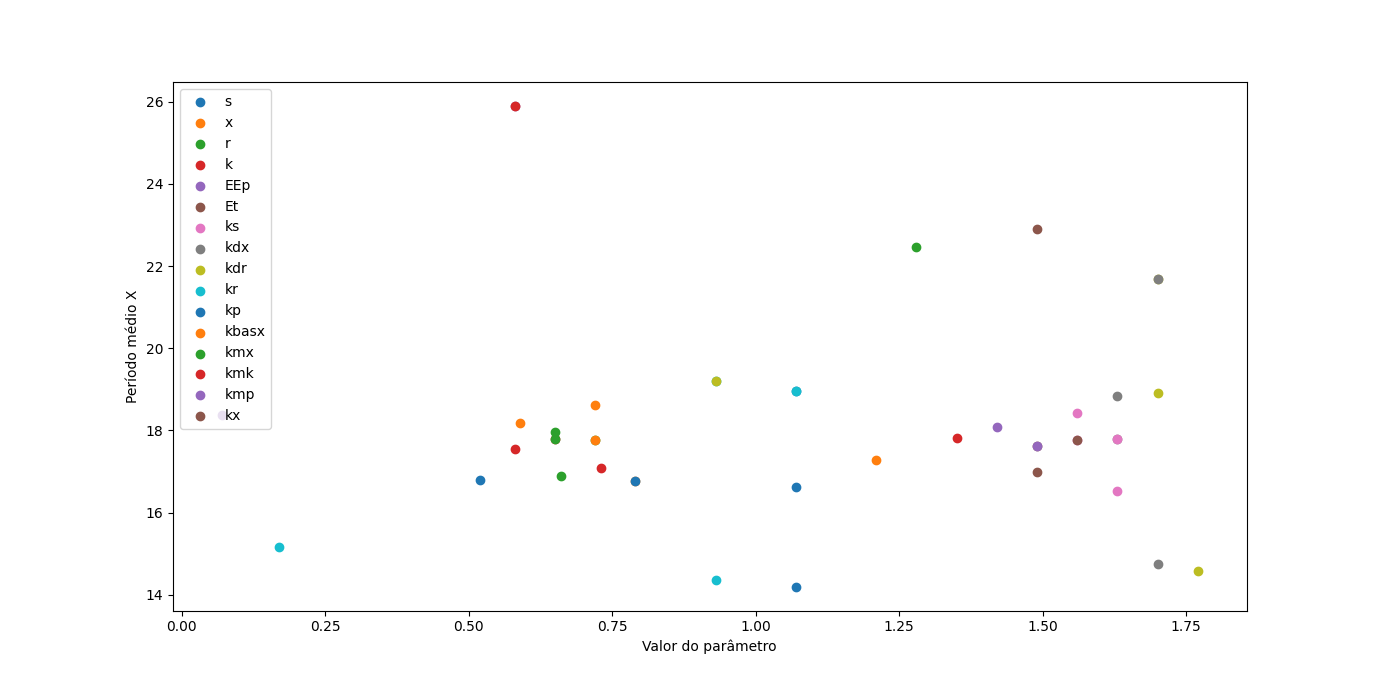
\includegraphics[width=16cm]{ParamsX.png}
			\caption{Gráfico de dispersão dos períodos encontrados para o composto X.}
			\label{fig}
		\end{center}
	\end{figure}
	
	\begin{figure}[hbtp]
		\begin{center}
			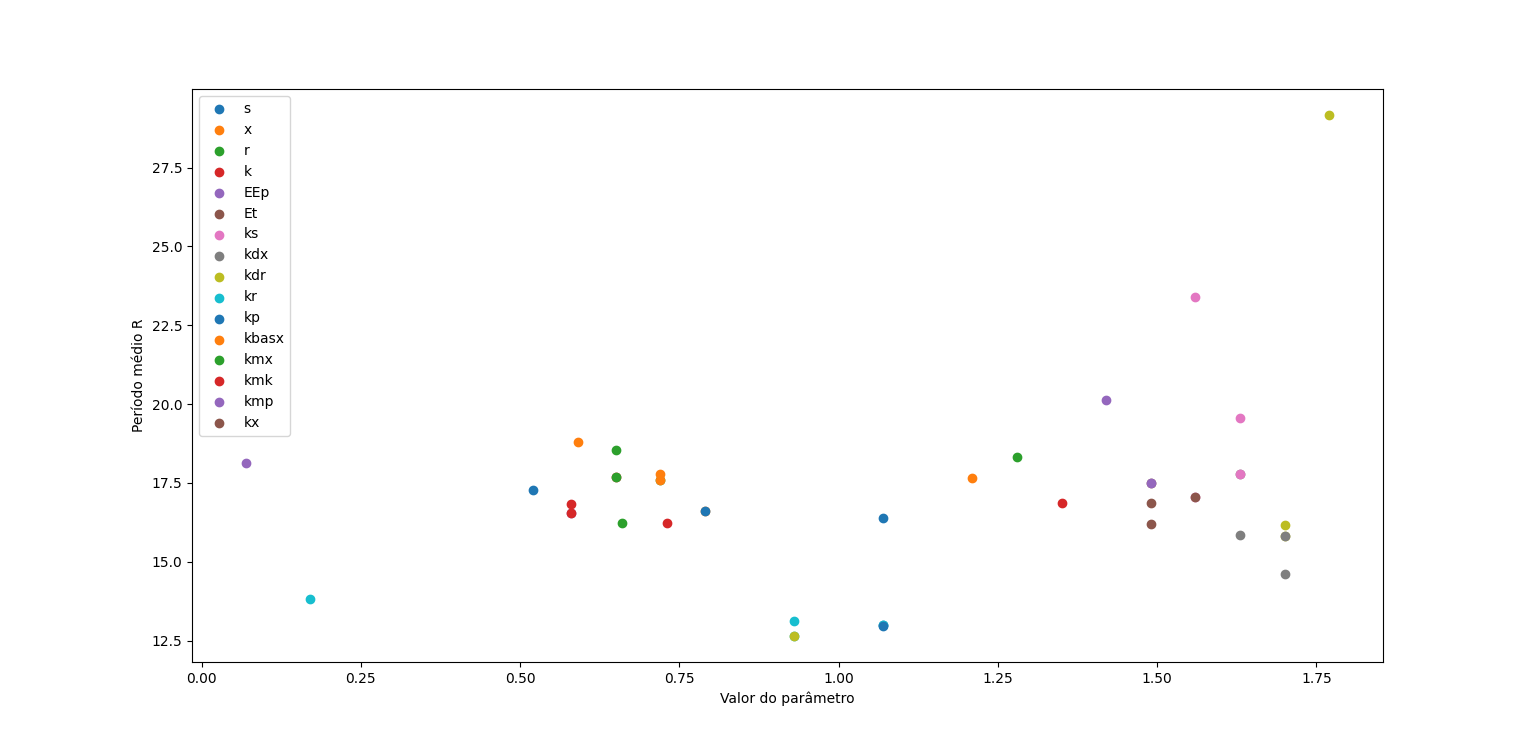
\includegraphics[width=16cm]{ParamsR.png}
			\caption{Gráfico de dispersão dos períodos encontrados para o composto R.}
			\label{fig}
		\end{center}
	\end{figure}
	
	\begin{figure}[hbtp]
		\begin{center}
			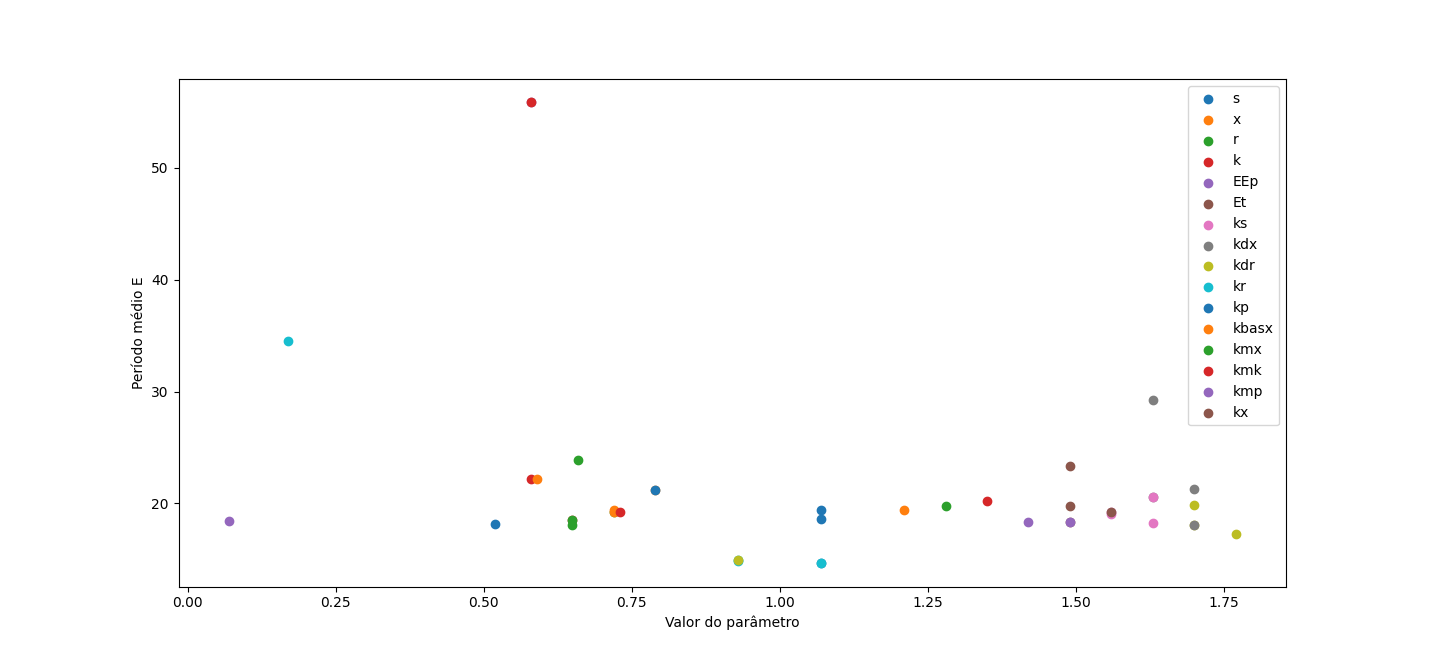
\includegraphics[width=16cm]{ParamsE.png}
			\caption{Gráfico de dispersão dos períodos encontrados para o composto E.}
			\label{fig}
		\end{center}
	\end{figure}
	\vspace{0.5cm}
	
	Por fim, aproveitando a série de adaptações que fiz por todas as funções, decidi amostrar aleatoriamente 3 casos do retorno de SearchPeriods e plotá-los assim como feito para a primeira execução, com o intuito de comprovar que as variações provocadas nos parâmetros podem gerar resultados relevantes. Esses plots são as figuras 17, 18 e 19.
	
		\begin{figure}[hbtp]
		\begin{center}
			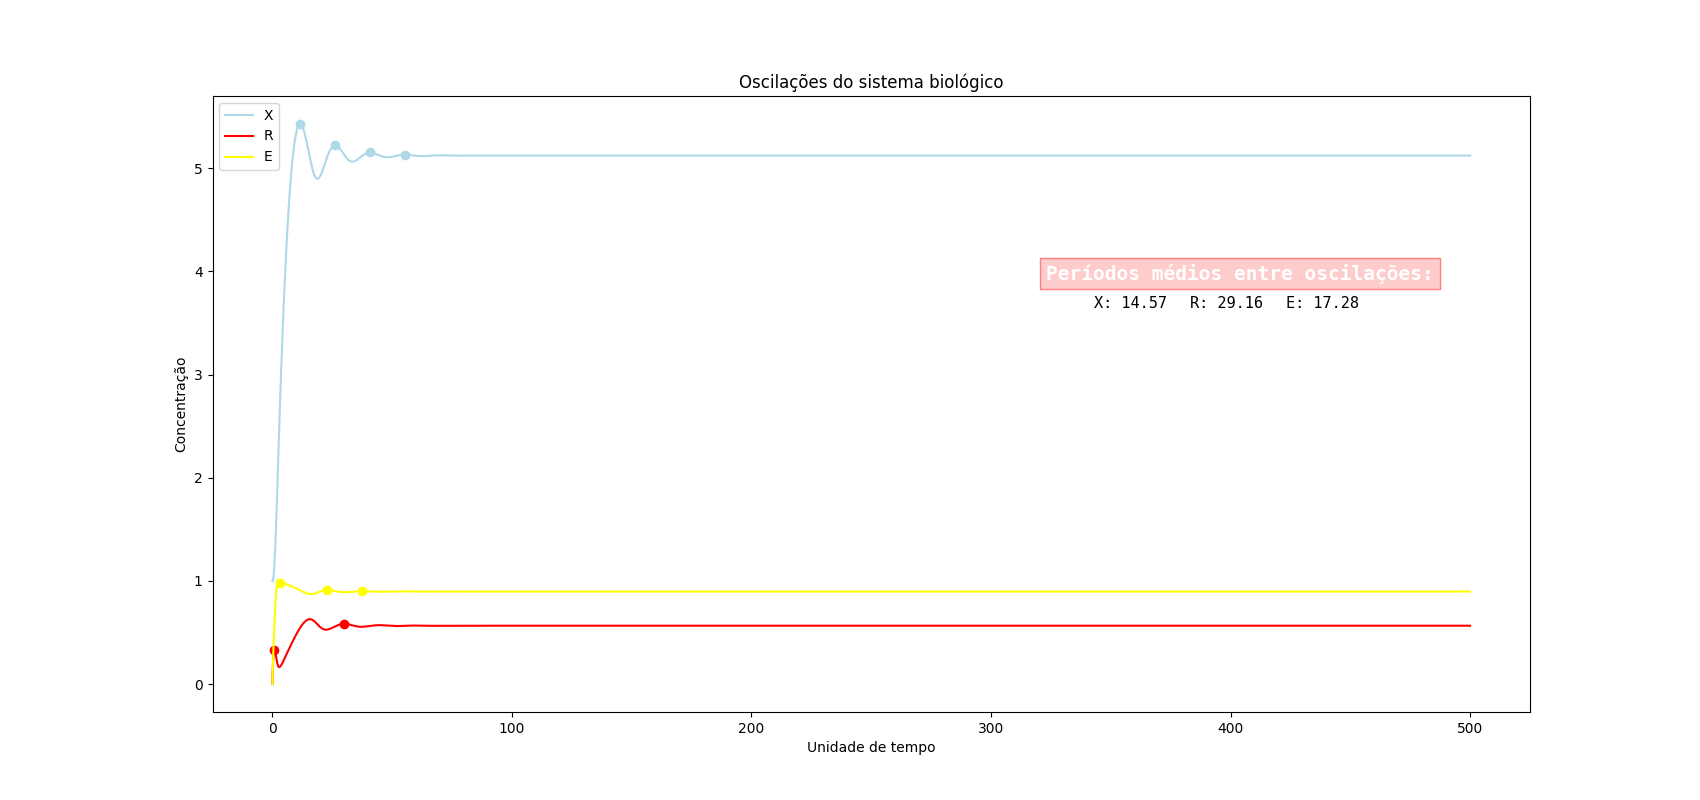
\includegraphics[width=16cm]{Sample1.png}
			\caption{Primeira amostra aleatória}
			\label{fig}
		\end{center}
	\end{figure}
	
	\begin{figure}[hbtp]
		\begin{center}
			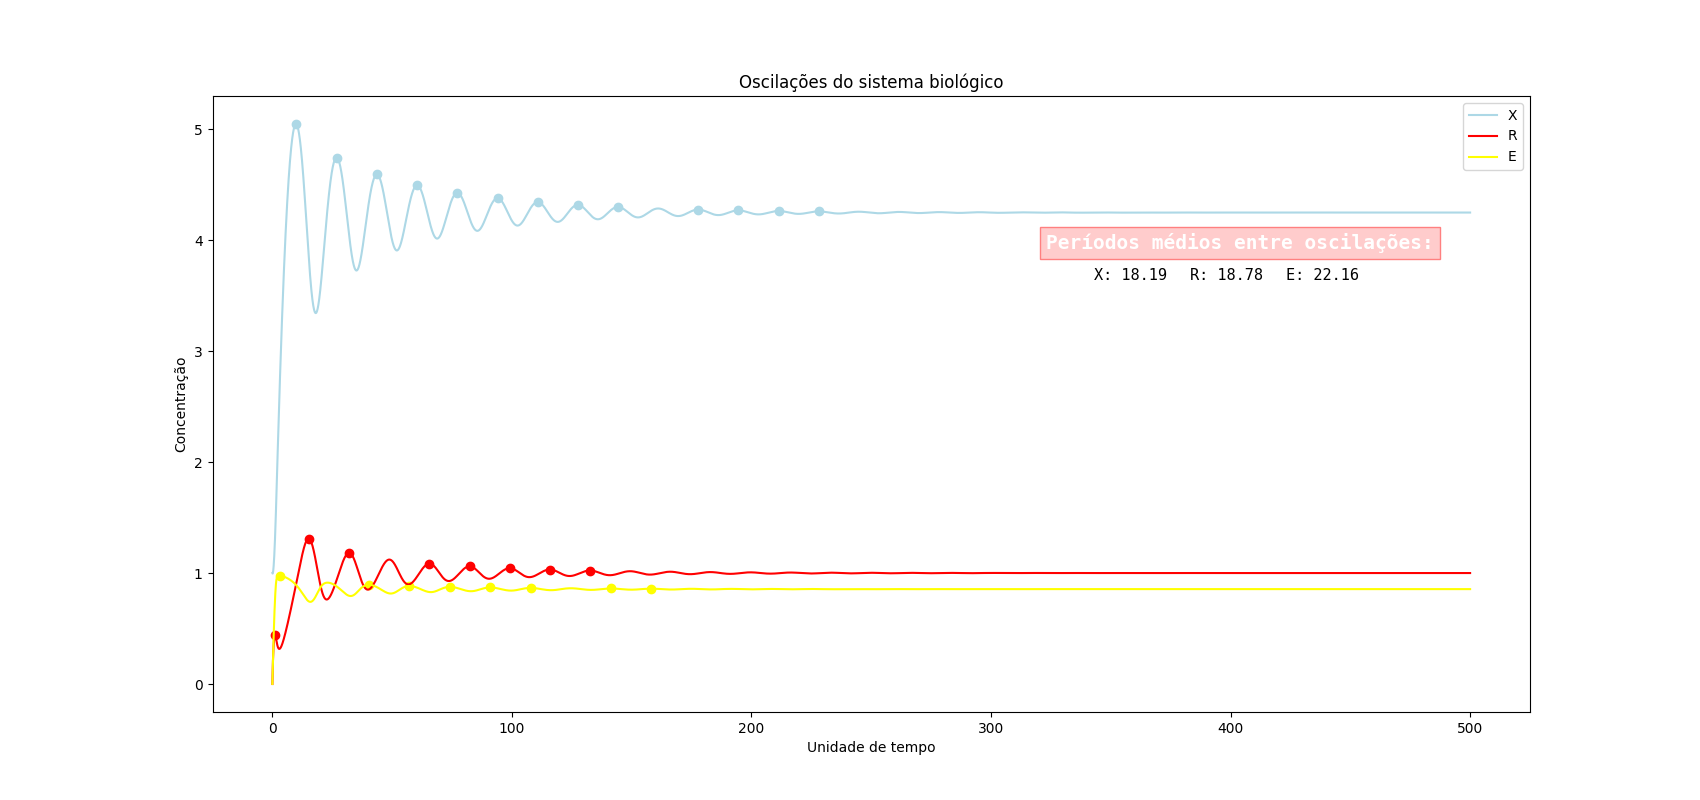
\includegraphics[width=16cm]{Sample2.png}
			\caption{Segunda amostra aleatória}
			\label{fig}
		\end{center}
	\end{figure}
	
	\begin{figure}[hbtp]
		\begin{center}
			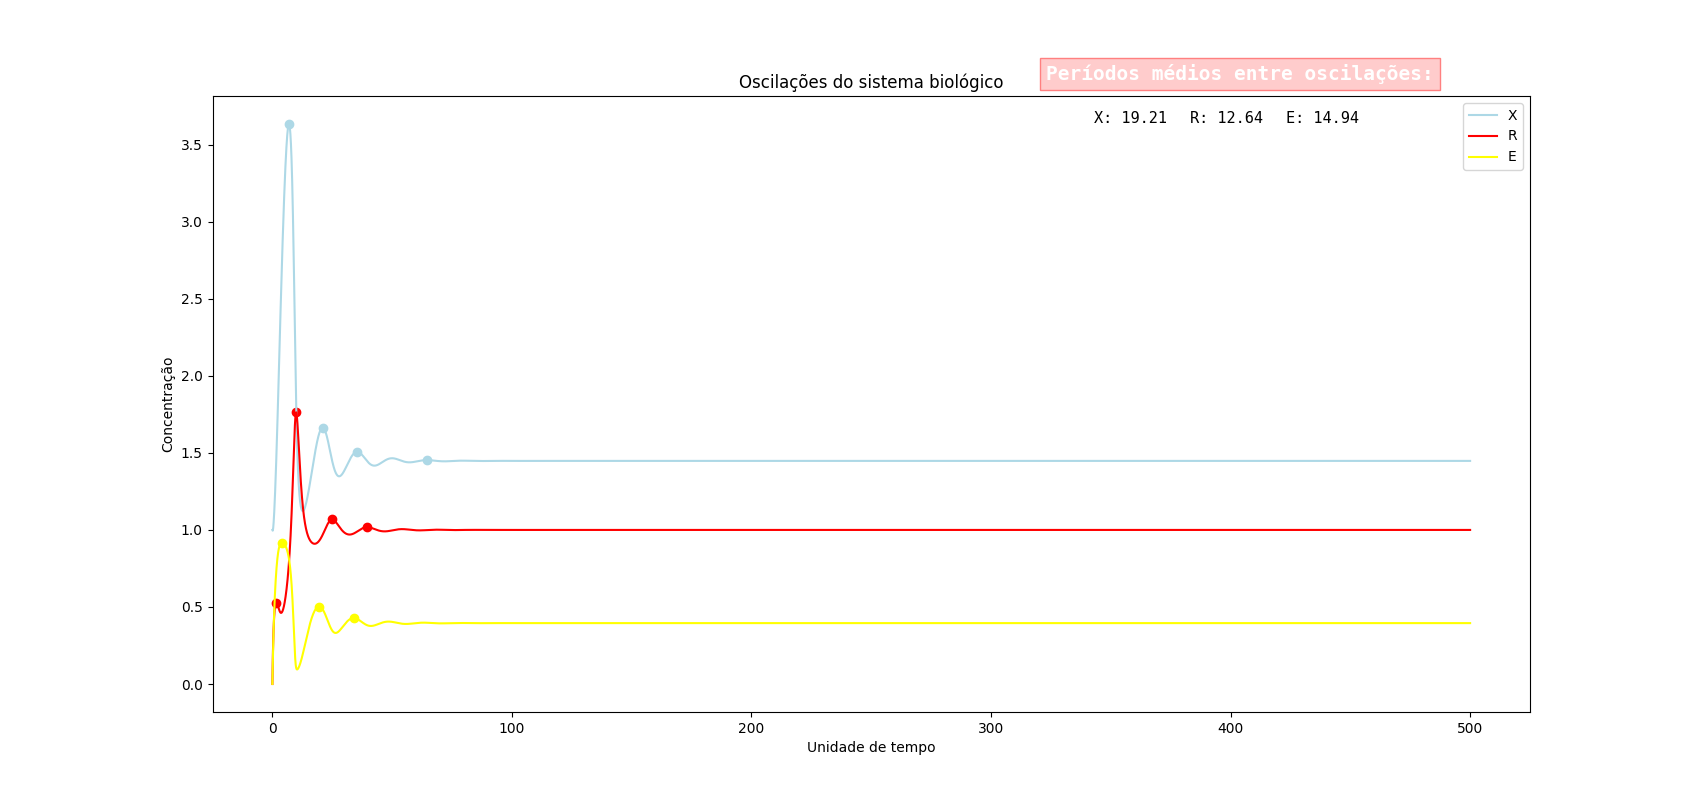
\includegraphics[width=16cm]{Sample3.png}
			\caption{Terceira amostra aleatória}
			\label{fig}
		\end{center}
	\end{figure}
	
	
	
	
	
	
	
	
	
	
	
	
	
	
	
	
	
	
	
	
	
	
	
	

	
	
	
	
	
	
	
	
	
	
	
\end{document}

